\section{CVaR model}

A CVaR bound of 0.0 indicates that CVaR is minimal, with 1.0 indicating that the optimization solely considers mean return.


\begin{figure}[tp]
\centering
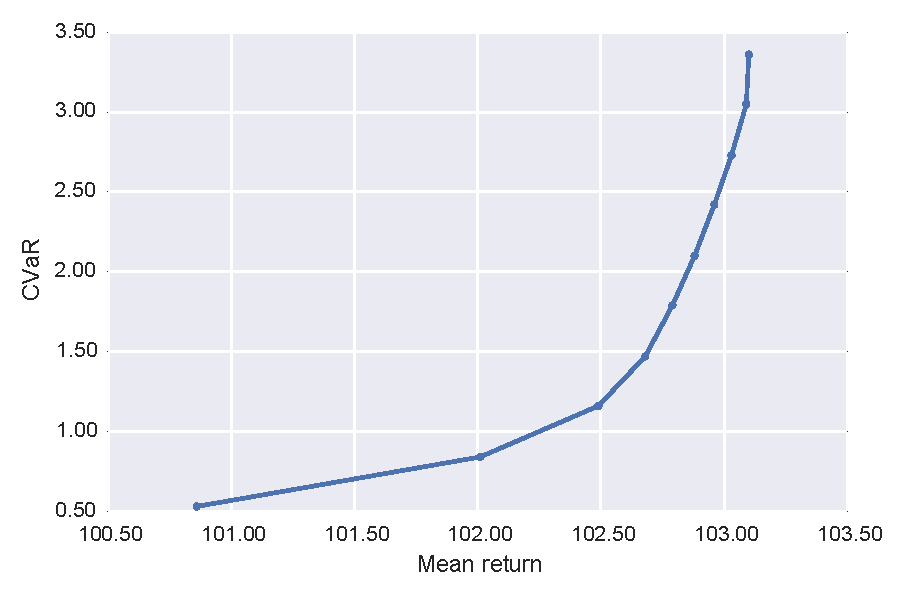
\includegraphics{../pic/frontier.pdf}
\caption{Optimal frontier for equidistant steps in CVaR.}
\label{fig:scenarioreturn}
\end{figure}

\begin{figure}[tp]
\centering
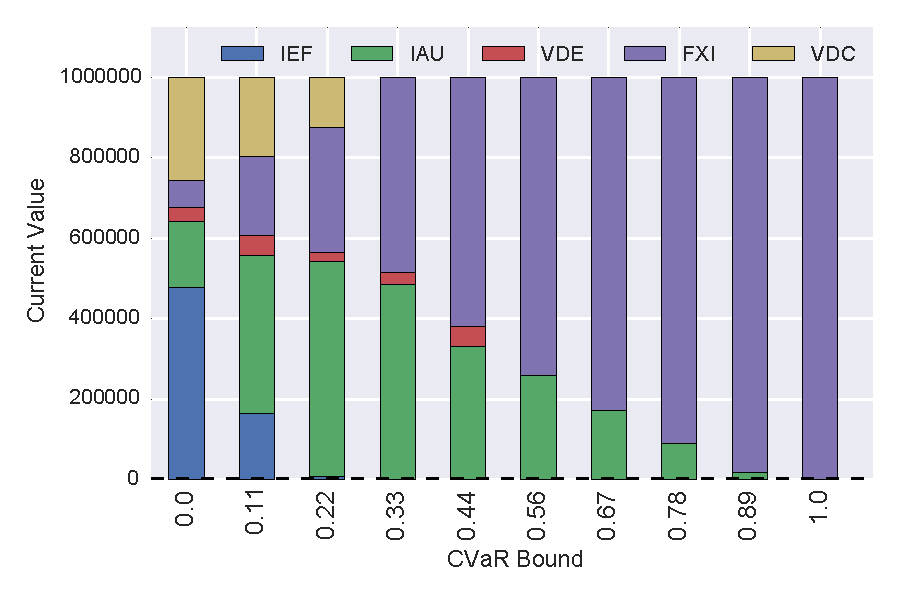
\includegraphics{../pic/Stake_vs_CVaR.pdf}
\caption{Portfolios at varying levels of the CVaR bound.}
\label{fig:scenarioreturn}
\end{figure}

\begin{figure}[tp]
\centering
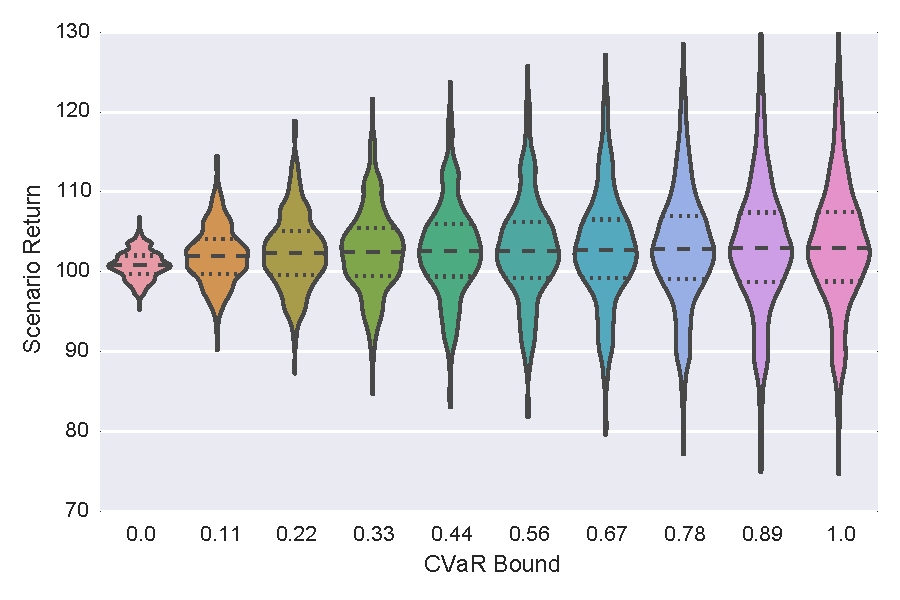
\includegraphics{../pic/Scenario_Return.pdf}
\caption{Scenario return for portfolios at varying levels of the CVaR bound.
The distributions for each bound are mirrored on the vertical axis, with the mean (dashed) and standard deviation (dotted) shown.}
\label{fig:scenarioreturn}
\end{figure}

Figure~\ref{fig:scenarioreturn} compares the scenario return at varying levels of the CVaR bound.